\documentclass[fleqn]{article}
\oddsidemargin 0.0in
\textwidth 6.0in
\thispagestyle{empty}
\usepackage{import}
\usepackage{amsmath}
\usepackage{graphicx}
\usepackage{flexisym}
\usepackage{calligra}
\usepackage{amssymb}
\usepackage{bigints} 
\usepackage[english]{babel}
\usepackage[utf8x]{inputenc}
\usepackage{float}
\usepackage[colorinlistoftodos]{todonotes}


\DeclareMathAlphabet{\mathcalligra}{T1}{calligra}{m}{n}
\DeclareFontShape{T1}{calligra}{m}{n}{<->s*[2.2]callig15}{}
\newcommand{\scriptr}{\mathcalligra{r}\,}
\newcommand{\boldscriptr}{\pmb{\mathcalligra{r}}\,}

\definecolor{hwColor}{HTML}{1a0252}

\begin{document}

  \begin{titlepage}

    \newcommand{\HRule}{\rule{\linewidth}{0.5mm}}

    \center


    \textsc{\LARGE Arizona State University}\\[1.5cm]

    \textsc{\LARGE Classical Parts/Field/Matter II}\\[1.5cm]


    \begin{figure}
      
\includegraphics[width=\linewidth]{asu.png}
    \end{figure}


    \HRule \\[0.4cm]
    { \huge \bfseries Problem Set 1}\\[0.4cm] 
    \HRule \\[1.5cm]

    \textbf{Behnam Amiri}

    \bigbreak

    \textbf{Prof: Maulik Parikh}

    \bigbreak


    \textbf{{\large \today}\\[2cm]}

    \vfill

  \end{titlepage}

  \begin{enumerate}
    \item If a charge is located at the coordinates $(2, -2, 1)$ and we are interested
    in some field at the point $(6, 3, 2)$, write down (in our and Griffiths’ notation)

      \textcolor{hwColor}{
        \hspace{10pt} Let's recall that a source point, $r^'$, is where an electric charge is located, and a field point, $r$, is which we
        are calculating the electric or magnetic field.
        \\
        \\
        Also, remember that 
        $
          \begin{cases}
            \overrightarrow{r} \equiv x \hat{x}+y \hat{y}+z \hat{z}
            \\
            \\
            \overrightarrow{\scriptr} \equiv r-r^'
            \\
            \\
            r=\sqrt{x^2+y^2+z^2}
          \end{cases}
        $
        \\
        \\
        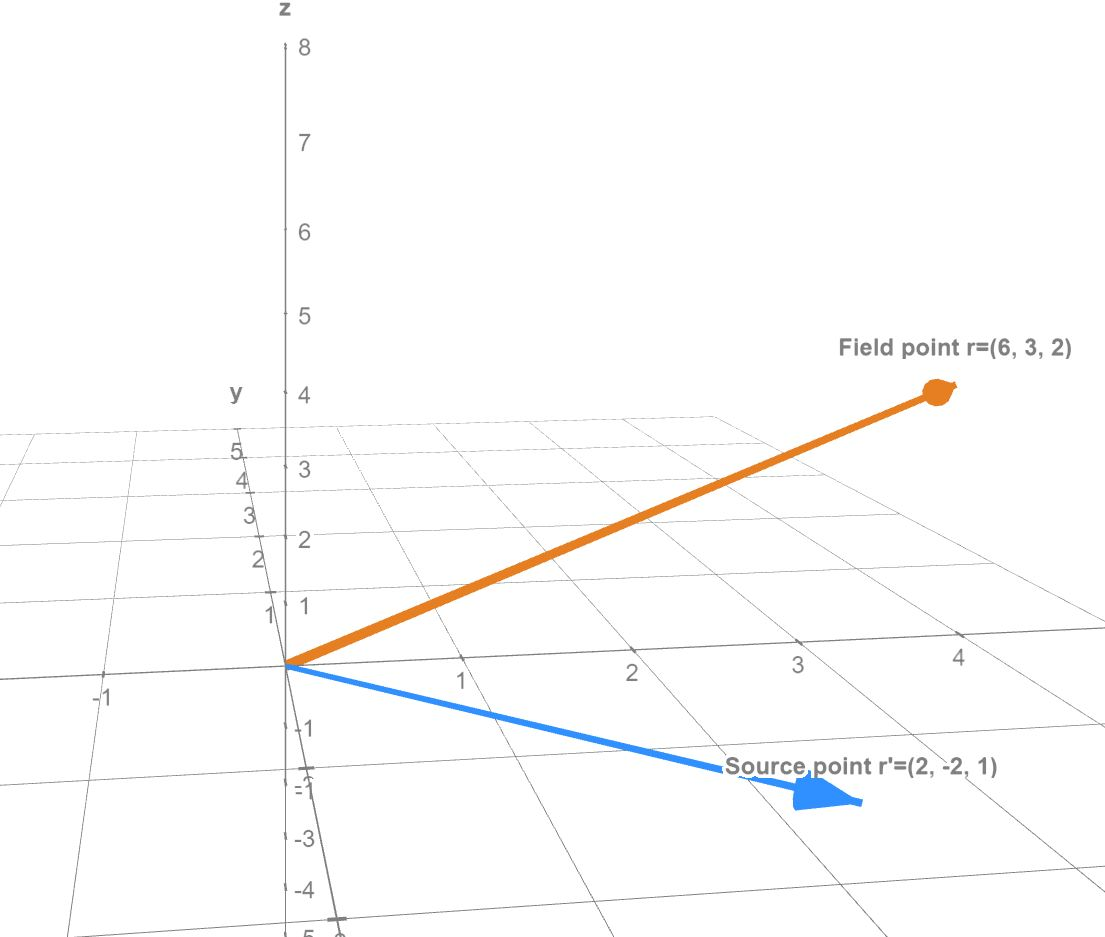
\includegraphics[height=8cm, width=8cm]{A.JPG}
      }
      

    \begin{enumerate}
      \item $\overrightarrow{r}$
      
        \textcolor{hwColor}{
          $
            \overrightarrow{r}=6 \hat{x}+3 \hat{y}+2 \hat{z}
          $
          \\
          \\
        }

      \item $\overrightarrow{r}^'$
      
        \textcolor{hwColor}{
          $
            \overrightarrow{r}^'=2 \hat{x}-2 \hat{y}+\hat{z}
            \\
            \\
          $
        }

      \item $\overrightarrow{\scriptr}$

        \textcolor{hwColor}{
          $
            \overrightarrow{\scriptr}=r-r^'=\left[ 
              \left(6 \hat{x}+3 \hat{y}+2 \hat{z}\right)-\left(2 \hat{x}-2 \hat{y}+\hat{z}\right)
            \right]
            \\
            \\
            \therefore ~~~ \overrightarrow{\scriptr}=4 \hat{x}+5 \hat{y}+\hat{z} 
          $
          \\
          \\
        }

      \item $r$

        \textcolor{hwColor}{
          $
            r=\sqrt{6^2+3^2+2^2}=\sqrt{49}
            \\
            \\
            \therefore ~~~ r=7
          $
          \\
          \\
        }
      
      \item $r^'$

        \textcolor{hwColor}{
          $
            r^'=\sqrt{2^2+(-2)^2+1^2}=\sqrt{9}
            \\
            \\
            \therefore ~~~ r^'=3
          $
        }

      \item $\scriptr$

        \textcolor{hwColor}{
          $
            \scriptr=|r-r^'|=\sqrt{4^2+5^2+1^2}
            \\
            \\
            \therefore ~~~ \scriptr=\sqrt{42}
          $
          \\
          \\
        }

      \item $\hat{r}$

        \textcolor{hwColor}{
          $
            \hat{r}=\dfrac{\overrightarrow{r}}{r}=\dfrac{6 \hat{x}+3 \hat{y}+2 \hat{z}}{7}
            \\
            \\
            \therefore ~~~ \hat{r}=\dfrac{6}{7} \hat{x}+\dfrac{3}{7} \hat{y}+\dfrac{2}{7} \hat{z}
          $
          \\
          \\
        }

      \item $\hat{r}^'$

        \textcolor{hwColor}{
          $
            \hat{r}^'=\dfrac{\overrightarrow{r}^'}{r^'}=\dfrac{2 \hat{x}-2 \hat{y}+\hat{z}}{3}
            \\
            \\
            \therefore ~~~ \hat{r}^'=\dfrac{2}{3} \hat{x}-\dfrac{2}{3} \hat{y}+\dfrac{1}{3}\hat{z}
          $
          \\
          \\
        }

      \item $\hat{\scriptr}$
      
        \textcolor{hwColor}{
          $
            \hat{\scriptr}=\dfrac{\overrightarrow{\scriptr}}{\scriptr}
            =\dfrac{4 \hat{x}+5 \hat{y}+\hat{z} }{\sqrt{42}}
            \\
            \\
            \therefore ~~~ \hat{\scriptr}=\dfrac{4}{\sqrt{42}} \hat{x}+\dfrac{5}{\sqrt{42}} \hat{y}+\dfrac{1}{\sqrt{42}} \hat{z} 
          $
          \\
          \\
        }

    \end{enumerate}

    \item Show that
    \begin{enumerate}
      \item $\overrightarrow{\nabla} \left(\dfrac{1}{\scriptr}\right)=-\dfrac{\hat{\scriptr}}{\scriptr^2}$

        \textcolor{hwColor}{
          $
            \overrightarrow{\nabla} \left(\dfrac{1}{\scriptr}\right)
            =\overrightarrow{\nabla} \left(\dfrac{1}{r-r^'}\right)
            =\overrightarrow{\nabla} \left(\dfrac{1}{\sqrt{(x-x^')^2+(y-y^')^2+(z-z^')^2}}\right)
            \\
            \\
            =\left(\dfrac{\partial}{\partial x} \hat{x}+\dfrac{\partial}{\partial y} \hat{y}+\dfrac{\partial}{\partial z} \hat{z}\right)
            .\left((x-x^')^2+(y-y^')^2+(z-z^')^2\right)^{-\dfrac{1}{2}}
            \\
            \\
            \\
            =\dfrac{\partial}{\partial x} \left((x-x^')^2+(y-y^')^2+(z-z^')^2\right)^{-\dfrac{1}{2}} \hat{x}
            \\
            +\dfrac{\partial}{\partial y} \left((x-x^')^2+(y-y^')^2+(z-z^')^2\right)^{-\dfrac{1}{2}} \hat{y}
            \\
            +\dfrac{\partial}{\partial z} \left((x-x^')^2+(y-y^')^2+(z-z^')^2\right)^{-\dfrac{1}{2}} \hat{z}
            \\
            \\
            \\
            =(-\dfrac{1}{2}) \left((x-x^')^2+(y-y^')^2+(z-z^')^2\right)^{-\dfrac{3}{2}} \dfrac{d}{dx} \left((x-x^')^2+(y-y^')^2+(z-z^')^2\right) \hat{x}
            \\
            +(-\dfrac{1}{2}) \left((x-x^')^2+(y-y^')^2+(z-z^')^2\right)^{-\dfrac{3}{2}} \dfrac{d}{dy} \left((x-x^')^2+(y-y^')^2+(z-z^')^2\right) \hat{y}
            \\
            +(-\dfrac{1}{2}) \left((x-x^')^2+(y-y^')^2+(z-z^')^2\right)^{-\dfrac{3}{2}} \dfrac{d}{dz} \left((x-x^')^2+(y-y^')^2+(z-z^')^2\right) \hat{z}
            \\
            \\
            \\
            =(-\dfrac{1}{2}) \left((x-x^')^2+(y-y^')^2+(z-z^')^2\right)^{-\dfrac{3}{2}} 2(x-x^') \hat{x}
            \\
            +(-\dfrac{1}{2}) \left((x-x^')^2+(y-y^')^2+(z-z^')^2\right)^{-\dfrac{3}{2}} 2(y-y^') \hat{y}
            \\
            +(-\dfrac{1}{2}) \left((x-x^')^2+(y-y^')^2+(z-z^')^2\right)^{-\dfrac{3}{2}} 2(z-z^') \hat{z}
            \\
            \\
            \\
            =-\dfrac{x-x^'}{\left((x-x^')^2+(y-y^')^2+(z-z^')^2\right)^{\dfrac{3}{2}}} \hat{x}
            \\
            -\dfrac{y-y^'}{\left((x-x^')^2+(y-y^')^2+(z-z^')^2\right)^{\dfrac{3}{2}}} \hat{y}
            \\
            -\dfrac{z-z^'}{\left((x-x^')^2+(y-y^')^2+(z-z^')^2\right)^{\dfrac{3}{2}}} \hat{z}
            \\
            \\
            \\
            =-\dfrac{\left[(x-x^')^2 \hat{x}+(y-y^')^2 \hat{y}+(z-z^')^2 \hat{z}\right]}{\sqrt{(x-x^')^2+(y-y^')^2+(z-z^')^2} . \left((x-x^')^2+(y-y^')^2+(z-z^')^2\right)}
            \\
            \\
            \\
            =-\dfrac{\dfrac{(x-x^')^2 \hat{x}+(y-y^')^2 \hat{y}+(z-z^')^2 \hat{z}}{\sqrt{(x-x^')^2+(y-y^')^2+(z-z^')^2}}}{(x-x^')^2+(y-y^')^2+(z-z^')^2}
            \\
            \\
            \\
            \therefore ~~~ \overrightarrow{\nabla} \left(\dfrac{1}{\scriptr}\right)=-\dfrac{\hat{\scriptr}}{\scriptr^2}
          $ 
        }

      \item $\overrightarrow{\nabla} . \left(\dfrac{\hat{\scriptr}}{\scriptr^2}\right)=4 \pi \delta^3 (\overrightarrow{\scriptr})$

        % \textcolor{hwColor}{
            
        % }

      \item $\overrightarrow{\nabla} \times \scriptr^n \hat{\scriptr}= \overrightarrow{0}$

        % \textcolor{hwColor}{
            
        % }

    \end{enumerate} 


    \item Using the product rules for vector derivatives (see inside cover of Griffiths) for a suitable product, show that
    \begin{enumerate}
      \item $\bigints\limits_{V} \left( \overrightarrow{\nabla} T \right) d\tau=\bigoint\limits_{S} T d\overrightarrow{a}$ where $T$ is a
      scalar function and $S$ is a surface bounding the volume $V$.
      
      


      \item $\bigints\limits_{S} \overrightarrow{\nabla} T \times d\overrightarrow{a}=-\bigoint\limits_{C} T d\overrightarrow{l}$ where $T$ is a scalar function 
      and $C$ is a curve bounding the surface $S$.



    \end{enumerate}

    \item A solid sphere of radius $R$ has uniform charge density $\rho$. Find the
    electric field $\overrightarrow{E}$ for all values of the radius $r$, both less than and greater
    than $R$.



    \item Consider a hollow ice cream cone placed upside-down with the tip or
    vertex of the cone on the positive $z$ axis. Suppose the cone has a halfangle of $\theta_0$ at the vertex 
    and that its height is $L$ (so the vertex is at $z=L$). If the cone has uniform surface charge density $\sigma$, what is the
    force on a charge $q$ placed at its tip?



    \item Suppose the semi-positive x-axis, $x\geq 0$, has linear charge density $\lambda$.
    Find the electric field at a point with $x=0$ but at a distance $L$ from the origin.


    \item  Let the electric field, expressed in spherical coordinates, be
    $$\overrightarrow{E}(\overrightarrow{r})=\dfrac{b}{r}\hat{r}
    +\dfrac{2b}{3r} sin(\theta) cos(\theta) sin(\phi) \hat{\theta}
    +\dfrac{b}{3r} sin(\theta) cos(\phi) \hat{\phi}$$
    where $b$ is some constant. Find the charge density $\rho(r, \theta, \phi)$.


    \item Look up the mass and charge of a proton and the values of the appropriate constants for this problem.
    \begin{enumerate}
      \item For a given separation $r$ between two protons, calculate the ratio
      of the magnitude of their electric repulsion to the magnitude of
      their gravitational attraction. That is why gravity is known as a
      weak force.


      \item Two protons in a helium nucleus are roughly $10^{-15}m$ apart. Calculate the force of 
      electric repulsion in Newtons. To put that in perspective, calculate the acceleration (in $m/s^2$) that a proton
      would feel. That is why the nuclear force that overcomes this repulsion is known as the strong force.


    \end{enumerate}

  \end{enumerate}

\end{document}